\documentclass{aci}

%%%%%%%%%%%%%%%%%%%%%%%%%%%%%%%%%%%%%%%%%%
\usepackage{txfonts}
\usepackage{cite}
\usepackage{booktabs}

\usepackage{hyperref}
\hypersetup{colorlinks=true}

%%%%%%%%%%%%%%%%%%%%%%%%%%%%%%%%%%%%%%%%%%
\newcommand{\ep}{\varepsilon}
\newcommand{\eps}[1]{{#1}_{\varepsilon}}

\def\typeofarticle{Research Article} \def\currentvolume{1} \def\currentissue{1}
\def\currentyear{2021} \def\currentmonth{} \def\ppages{1--30} \def\DOI{to
appear} \def\Received{June 2022} \def\Accepted{July 2022} \def\Published{October
2022 }
%\numberwithin{equation}{section}
\DeclareMathOperator*{\essinf}{ess\,inf}

%%%%%%%%%%%%%%%%%%%%%%%%%%%%%%%%%%%%%%%%%%
\begin{document}

\title{An Ant Cuticle Texture Classification Algorithm for Ecological Anaylsis}

\author{%
  Noah Gardner\affil{1}, John Paul Hellenbrand\affil{2}, and Chih-Cheng
  Hung\affil{1}\corrauth}

% \shortauthors is used in copyright information in the end of the paper
\shortauthors{the Author(s)}

\address{%
  \addr{\affilnum{1}}{College of Computing and Software Engineering, Kennesaw
    State University, 1000 Chastain Road, Kennesaw, GA 30144, USA; email}
  \addr{\affilnum{2}}{College of Science and Mathematics, Kennesaw State
    University, 1000 Chastain Road, Kennesaw, GA 30144, USA; email}}
% corresponding author
\corraddr{chung1@kennesaw.edu}

\editor{First-name Last-name}

\begin{abstract}
  There is a large variety of ant species, and most species are diverse in terms
  of size, shape, behaviors, and especially skin (cuticle) textures. However,
  the significance of ant cuticle texture is not widely researched. This
  research employs modern machine learning methods such as texture analysis and
  classification with CNN and clustering to automatically group similar ant
  species to allow for the study of influences cuticle texture on ant ecology.

\end{abstract}

\keywords{Texture Analysis, Image Processing, Clustering, Machine Learning,
  Myrmecology, Ecology}

\maketitle
\section{Introduction}
Insects compose half of biodiversity and rank among the most dominant organisms
in terrestrial ecosystems \cite{sheikh_diverse_2017}. A key factor for the
ecological success of insects is their exoskeleton, also known as cuticle. The
cuticle protects insects from predation, provides structural support, prevents
desiccation, and serves as a canvas for advertising visual and chemical signals
\cite{gullan_insects_2009}. Research has heavily focused on the macrostructures
and internal chemical components that make the exoskeleton functional and more
recent work is being done to understand the functional aspects of external
cuticle micro sculpturing \cite{muthukrishnan_insect_2020,
  gunderson_insect_1989, watson_diversity_2017}.

Texture is an important feature in many applications, such as image processing,
pattern recognition, and computer vision. Analysis of textures can be broken
into three main categories: texture classification, texture segmentation, and
texture synthesis \cite{reed_review_1993}. The process of classifying a texture
into a set of categories and relies on three different approaches. In this
paper, we focus on a \textit{model-based approach} which attempts to extract
parameters to reveal common patterns and use those parameters to automatically
distinguish between different textures \cite{maillard_texture_2003}.

Although there is some work regarding grouping ants into categories of similar
cuticle, automated classification has yet to become an active area of research.
Due to the large number of different ant species, the classification of ants
into categories of similar texture is difficult to accomplish manually. Texture
analysis has shown promising results in related fields, such as plant
identification \cite{boudra_plant_2018}. With modern texture analysis methods,
the classifications of ants can be automated and the results can be used to
study the influence of cuticle texture on ant ecology.

We examine ants (\textit{Formicidae}) as they display an extreme diversity of
cuticle micro sculpturing across all subfamilies. Sculpturing ranges from
parallel longitudinal ridges to deep oval impressions to erratic protuberances.
The sculpturing has arisen convergently and independently throughout ant’s
evolutionary history, which suggests some inherent function. Cuticle sculpturing
on ants may help increase strength and rigidness, resist abrasion, increase
internal and external surface area, resist microbial growth, and rear beneficial
anti-biotic producing bacteria \cite{johnson_effect_2011,
  bruckner_relationship_2017, currie_coevolved_2006}. These specific functions may
be associated with certain sculpturing types and the purpose of classification
is to group similar textures based on proposed function.

\section{Related Work}
Taxonomists have developed extensive terminology describing ant cuticle
sculpturing as it is often a useful diagnostic trait to distinguish between
closely related ant species \cite{blaimer_taxonomy_2019,fisher_ants_2007}. The
definitive text on ant cuticle terminology — \textit{The Glossary of Surface
  Sculpturing} — contains over 100 terms to describe the cuticle sculpturing
patterns of ants \cite{harris_glossary_1979}. There is often substantial overlap
among terms, and closely related cuticle patterns are likely to be functionally
similar. For example, the definition for “imbricate” is, “partly overlapping and
appearing like shingles on a roof or scales on a fish,” which is difficult to
distinguish from the definition of tesselate, “made up of squares like a chess
board, either in sculpturing or in color.”

Cuticle sculpturing in ants has been explored thoroughly from a taxonomic
perspective; however, the function of nano and microstructures on insect
exoskeletons is a developing topic in entomology. Watson et al. reviews the
literature of cuticle nano and microstructure function and proposes 21 possible
functions associated with these structures \cite{watson_diversity_2017}. Many of
these functions are related to structures not found in ants such as scales and
nanostructures. The review does include functions that may relate to ants such
as friction control, enhanced surface area, and increased hardness.  Watson et
al. also describe seven types of cuticle structures ranging from hairs and
scales to nano and micro structures \cite{watson_diversity_2017}. The cuticle
sculpturing of ants seems to fall within one type – complex microstructures.

The five broad functional groupings developed that describes the complex
microstructures found on ants were derived from reviewing the variation of
cuticle sculpturing across ants. These functional groupings were also reflected
in Harris as many terms could be grouped together based on similar definitions
and comparing the SEM photographs provided in the publication
\cite{harris_glossary_1979}.


\section{Proposed Approach}

\section{Methods}

\subsection{Sculpture Identification Protocol}
A team of three assistants were in charge of the manual identification process.
The team was trained to identify cuticle sculpturing through a process which
consisted of one 45-minute introductory lesson explaining the project and
texture categories and then given a training set of photos to identify from the
genus \textit{Polyrhachis}, whose members display among the highest diversity of
cuticle patterns all categories. The training set identifications were reviewed
together as a group. Once training was complete, assistants were assigned the
same genera of ants to identify independently each week. A weekly meeting was
held to discuss identifications and assign new ones. These identifications were
collected in a spreadsheet and the identifications were assigned to individual
ant species on a majority basis.

\subsection{Dataset}
In order to classify the cuticle, we used ant head images sourced from AntWeb
\cite{perrichot_antweb_2012}. In general, the ant head images are centered in
the image, facing the front, and share a similar posture. However, some images
may not be centered, show the ant head in a different orientation, or may have a
drastically different resolution from the average image. Fortunately, each can
have several scales available such that the images' scales can be roughly
similar.

\begin{table}[ht]
  \centering
  \caption{Dataset Subclass Distribution}
  \label{table:classdist_all_full}
  \begin{tabular}{lll}
\toprule
Label & Samples (n) & Samples (\%) \\
\midrule
Rough Dimpled  &         173 &        0.07 \\
Rough Netted   &         503 &        0.21 \\
Rough Ridged   &         317 &        0.13 \\
Rough Tuberous &          41 &        0.02 \\
Smooth Gritty  &          16 &        0.01 \\
Smooth         &        1393 &        0.57 \\
Total          &        2443 &         1.0 \\
\bottomrule
\end{tabular}

\end{table}

\begin{table}[ht]
  \centering
  \caption{Dataset Class Distribution}
  \label{table:classdist_rs_full}
  \begin{tabular}{lll}
\toprule
{} & Samples (n) & Samples (\%) \\
\midrule
Rough  &        1034 &        0.42 \\
Smooth &        1409 &        0.58 \\
Total  &        2443 &         1.0 \\
\bottomrule
\end{tabular}

\end{table}

Images were collected and classified by according to the sculpturing
identification protocol. Overall, there are a total of 2443 images in the
dataset. The class distribution with all considered subclasses is shown in Table
\ref{table:classdist_all_full}, and the class distribution with overall
distribution is shown in Table \ref{table:classdist_rs_full}. The relatively
small number of images in the dataset paired with the uneven class distribution
makes it difficult to perform a meaningful classification. However, the goal of
this project is to develop a classification algorithm that can be used to help
classify over 200,000 ant images. Therefore, it is desirable to use a few
representative images from each class to train the algorithm. Additionally, data
augmentation and other methods are performed to increase the number of training
images to create a more robust classification algorithm.

\subsection{Subimage Dataset}

\begin{figure}[ht]
  \centering
  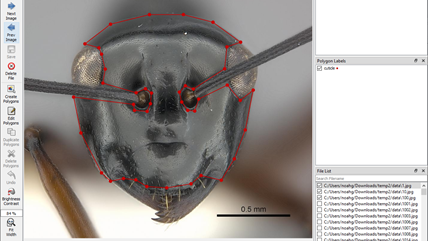
\includegraphics[width=0.8\textwidth]{assets/images/segmented_1.png}
  \caption{Hand segmented ant head image to separate head cuticle from other
    sections of the image.
    \href{https://www.antweb.org/bigPicture.do?name=casent0217419&shot=h&number=1}{CASENT0217419}
    by \href{https://www.antweb.org/artist.do?id=92}{Estella Ortega}, from
    \href{https://www.antweb.org}{AntWeb}, is licensed under
    \href{https://creativecommons.org/licenses/by/4.0/}{CC BY 4.0}}
  \label{fig:segmented_1}
\end{figure}

When using the Sculpture Identification Protocol, the class of the overall image
is based only on the texture of the head, not the eyes, antenna, or any other
exposed cuticle. We use image segmentation to analyze the texture by splitting
the ant head image into a set of regions: \textit{cuticle} and
\textit{background}. A benefit of this approach allows us to pull patches or
subimages of various sizes from the region to increase the number of samples
available for training and at the same time, reduce the number of features to
simplify the classification algorithm. With a given subimage size to extract
from the segmented image, we label each subimage extracted based on the class of
the input image. Overall, there are 73 images that were hand segmented in this
manner and the class distribution for various sizes of subimages are shown in
Table \ref{table:classdist_rs_sub}.

\begin{table}[ht]
  \centering
  \caption{Subimage Dataset Class Distribution}
  \label{table:classdist_rs_sub}
  \begin{tabular}{lllll}
\toprule
Label &  (8, 8) & (16, 16) & (24, 24) & (32, 32) \\
\midrule
Rough  &  101584 &    23655 &     9790 &     5108 \\
Smooth &  104981 &    24356 &    10022 &     5177 \\
Total  &  206565 &    48011 &    19812 &    10285 \\
\bottomrule
\end{tabular}

\end{table}

\section{Experimental Results}

\subsection{Sculpturing Identification}
In our initial trial, we examined the entire \textit{Polyrhachis} genus, which
was 581 eligible specimens out of the 775 species. 71\% of the classifications
were unanimous. We then expanded our categorizations to 2846 images of
individual species from 13 genera. These genera were from the four major ant
subfamilies Ponerinae, Myrmicinae, Formicinae, and Dolichoderinae along with
Dorylinus and Ectatomminae. 87\% (2486) of classifications were unanimous. This
percentage represents the accuracy for the entirety of identifications starting
November 2020 and ending in March 2021. Assistants were also asked to complete
an ant cuticle assessment near the end of the identification process. The
assessment consisted of images from forty species of ants that spanned all
categories. The purpose of the assessment was to measure the consistency of
identifications while removing any biases from weekly meeting discussions and
cross referencing of other identifications. Unanimous classification was reached
90\% of the time during the individual assessment.

Classifications became more consistent overtime. One likely reason for this
increase was that students gained additional experience in cuticle
classification over the course of these trials. However, definitions of cuticle
texture categories were refined overtime. At the inception of the project,
assistants based classifications off of reference photos and tentative
definitions that were sometimes unclear. For example, striate was initially
defined as “long linear ridges, corresponding in-between ridges vary in length.”
Also, some tentative categories had low agreement amongst the team. For example,
striate initially was a broad category containing two subclasses (Severe and
Mild) and encompassed longitudinal and latitudinal ridges. Based on several
rounds of feedback from students and identification of these problem categories
where there was low agreement, the definitions developed into the current
classification system.

\subsection{Binary Classification}

In the first experiment, we investigate the ability of a basic CNN to classify
cuticle texture into the two main categories: \textit{rough} and
\textit{smooth}. The goal of this experiment is to determine if more intricate
data preprocessing or a more powerful model is necessary to classify the texture
of the ant. Images were resized to different sizes for CNN input and different
samples per class were also tested. The dataset used is shown in Table
\ref{table:classdist_rs_full}, and the results are shown in Table
\ref{table:exp1_full}.

\begin{table}[ht]
  \centering
  \caption{Binary Classification of Full Size Images}
  \label{table:exp1_full}
  \begin{tabular}{llrr}
\toprule
      Size & Samples (per class) &  Accuracy (avg) &  Loss (avg) \\
\midrule
  (64, 64) &                 250 &            70.8 &       0.705 \\
  (64, 64) &                 500 &            74.9 &       0.763 \\
  (64, 64) &                 750 &            76.7 &       0.712 \\
(128, 128) &                 250 &            71.9 &       0.977 \\
(128, 128) &                 500 &            74.4 &       1.133 \\
(128, 128) &                 750 &            75.7 &       1.137 \\
(256, 256) &                 250 &            71.0 &       1.353 \\
(256, 256) &                 500 &            73.3 &       1.532 \\
(256, 256) &                 750 &            75.0 &       1.504 \\
(512, 512) &                 250 &            68.2 &       1.790 \\
(512, 512) &                 500 &            71.2 &       1.625 \\
(512, 512) &                 750 &            71.7 &       1.852 \\
\bottomrule
\end{tabular}

\end{table}

\section*{Acknowledgments}
We would like to thank the constructive feedback provided by the reviewers.

\bibliography{paper}
\bibliographystyle{unsrt}

\end{document}
